\documentclass[a4paper,10pt, openright]{book}%{report}
\usepackage[utf8]{inputenc}
\usepackage[italian]{babel}
\usepackage{amsmath}
\usepackage{amsfonts}
\usepackage{amssymb}
\usepackage{amsthm}
\usepackage{graphicx}
%\usepackage[left=2cm,right=2cm,top=2cm,bottom=3cm]{geometry}
\usepackage{bigfoot}
\usepackage{bold-extra}

\usepackage[numbers]{natbib}

\usepackage{hyperref}
\hypersetup{colorlinks, linkcolor=blue}




\theoremstyle{plain}% default
\newtheorem{thm}{Teorema}[section]
\newtheorem{lem}[thm]{Lemma}
\newtheorem{prop}[thm]{Proposizione}
\newtheorem{assu}[thm]{Assunzione}
\newtheorem{cor}{Corollario}
\theoremstyle{definition}
\newtheorem{defi}{Definizione}[section]
\newtheorem{conj}{Congettura}[section]
\newtheorem{exmp}{Esempio}[section]
\theoremstyle{remark}
\newtheorem{oss}{Osservazione}
\newtheorem*{note}{Nota}
\newtheorem*{case}{Caso}

\setcounter{secnumdepth}{3}

\newcommand{\pk}{\textit{PK} } 
\newcommand{\mk}{\textit{MK} }
\newcommand{\evil}[1]{$\mathcal{#1}$}
\DeclareMathOperator{\parent}{parent}
\DeclareMathOperator{\att}{att}
\DeclareMathOperator{\inde}{index}
\DeclareMathOperator{\num}{num}

\DeclareMathOperator{\decrypt}{DecifraNodo}
\DeclareMathOperator{\polysat}{PolySat}
\DeclareMathOperator{\polyunsat}{PolyUnsat}


\begin{document}
\frontmatter
\begin{titlepage}
\begin{center}
{{\Large{\textsc{Università degli Studi di Trento}}}}
\rule[0.1cm]{15.8cm}{0.1mm}
\rule[0.5cm]{15.8cm}{0.6mm}
{\small{\textsc { Dipartimento di Matematica \\
Corso di Laurea in Matematica}}}
\end{center}
\begin{center}
\begin{figure}[!htbp]

\includegraphics[scale=0.35]{unitn.jpg} \centering 
\centering
\end{figure}
\vspace{10mm}
\begin{center}
{\LARGE{\bf \-}}\\
\vspace{3mm}
{\LARGE\textbf{Attributive Based Encription}}\\
\vspace{3mm}
{\LARGE{\bf \-}}\\
\vspace{3mm}
{\LARGE{\bf --}}\\
\vspace{7mm} {\large{\sc Elaborato Finale}}
\end{center}
\vfill
\par
\noindent
\begin{minipage}[t]{0.47\textwidth}
{\large{\sc Relatore: Prof.}\\
{ \\ Andrea Caranti}}\\
\end{minipage}
\hfill
\begin{minipage}[t]{0.47\textwidth}\raggedleft
{\large{\sc Laureando:}\\ 
\vspace{5mm} 
{ Carlo Brunetta}}
\end{minipage}
\vspace{20mm}
\begin{center}
{\large{\sc Anno Accademico 2013/2014}}
\end{center}
\end{center}
\end{titlepage}

\thispagestyle{empty}

\newpage
\thispagestyle{empty}
\begin{flushleft}
\textit{Eventuale proposizione}\\
\end{flushleft}
\vspace*{3cm}
\begin{flushright}
Eventuale dedica
\end{flushright}

\newpage
\tableofcontents
\newpage
\mainmatter

\section*{Abstract}
Ultra-Riassunto:\\
Citare \cite{kpabe} e poi riassumenre l'intro


\chapter{Introduzione}




\begin{itemize}
	\item Differenza tra keying e pairing
	\item \cite{nict} c'è un trafiletto interessante su cui discutere
	\item Cosa vogliamo ottenere (documento a più ingressi, idea)
	\item I Functional Encryption \cite{cse}
	\item IBE e ABE
\end{itemize}


% \section{Ambiente}


% {\bfseries
% Molte volte c'è la necessità di scambiare informazioni segrete ad un gruppo di persone ben definito. Gli attuali metodi di crittografia largamente utilizzati necessitano di scambiare la propria chiave privata con tutti i vari membri del gruppo che riesce così a decriptare ogni messaggio criptato per questa chiave.

% Il nostro scopo è di sviluppare un metodo capace di fornire chiavi \emph{ad hoc} che permettano la decifratura solo se vengono rispettati dei parametri decisi da chi cripta il messaggio. In questo modo possiamo garantire l'accesso alle informazioni unicamente a gruppi ben mirati di persone.

% Vogliamo che il sistema ci garantisca di non ottenere chiavi ad accessi più deboli ma che si possano generare chiavi più forti partendo dalle proprie chiavi. ( es. $A $and $B$ e $B$ and $C$ non ci permette di creare una chiave $B$)
 
% \begin{itemize}
% \item Sviluppo storico della crittografia (breve) e spiegazione della necessità di metodi potenti di cifratura
% \item Idea del metodo crittografico KP-ABE
% \item Differenze da altri metodi
% \end{itemize}}

% \subsection{Finalità} 

% \textbf{Cosa vogliamo ottenere da questo metodo di crittografia?}



% \section{Strumenti algebrici}
% \begin{defi}
% Un gruppo ciclico e il suo generatore
% \end{defi}
% \textbf{Definizioni minime e spiegazione di cosa serve a noi. Piccola digressione sui gruppi sulle curve elittiche}

% \begin{defi}
% Sia $G_1,G_2$ gruppi ciclici di ordine $p,q$ primi. Sia $g$ un generatore.\\
% Sia $e : G_1 \times G_1 \rightarrow G_2$ una mappa bilineare con proprietà:
% \begin{enumerate}
% \item $e$ è bilineare rispetto al prodotto
% \[ \forall_{u,v \in G_1}, a,b \in \mathbb{Z}_p : e(u^a,v^b) = e(u,v)^{ab} \]
% \item $e$ è non degenere \[e(g,g) \neq 1\]
% \item $e$ è velocemente computabile
% \end{enumerate}
% \end{defi}
% \textbf{Qualche esempio magari in un qualche contesto ben fatto.}

% \begin{defi}
% Coefficente di Lagrange
% \[ \Delta_{i,s}(x) = \prod_{j\in S , j \neq i} \dfrac{x-j}{i-j} \]
% \end{defi}

% \begin{defi}
% Funzione di soglia : \href{http://www.contrib.andrew.cmu.edu/~ryanod/?p=856}{link per def.} 
% \end{defi}
% \textbf{Forse troppo generale. Esempio partendo da funzioni booleane.}


% \begin{prop}
% Legame
% \[\sum_z \Delta_{i,s_x^\prime(0)} = 1\]
% \end{prop}
% \textbf{Legame trovato, basta considerare delle proprietà dell'insieme su cui si fa la sommatoria}

% \begin{prop}
% Completamento di polinomi \textbf{che vengono utilizzati spesso e lasciati in maniera molto sbrigativa.} 
% \end{prop} 

\chapter{Attribute Based Encryption}

ABE (Attribute Based Encryption) è una famiglia di schemi di crittografia basati tutti sull'utilizzo di una mappa bilineare e non degenere $e:G_1 \times G_2 \rightarrow G_3$ con $G_i$ gruppi ciclici di ordine un numero primo.

Questa famiglia può esser suddivisa in due sotto-famiglie che si differenziano sul processo di autorizzazione per la decifratura :
\begin{itemize}
	\item \textbf{{Chipertext Policy ABE}} :  Il messaggio cifrato contiene le regole d'autorizzazione. L'autorizzazione viene concessa se la chiave private dell'utente soddisfa la policy del messaggio.
	\item \textbf{Key Policy ABE} : La chiave dell'utente contiene le informazioni sulla policy d'autorizzazione. Il messaggio cifrato conterrà gli attributi necessari per permettere la decodifica.
\end{itemize}

\begin{minipage}[c]{0.9\textwidth}
\vspace{0,3cm}
\centering
	\begin{minipage}[c]{0.45\textwidth}
		\centering
		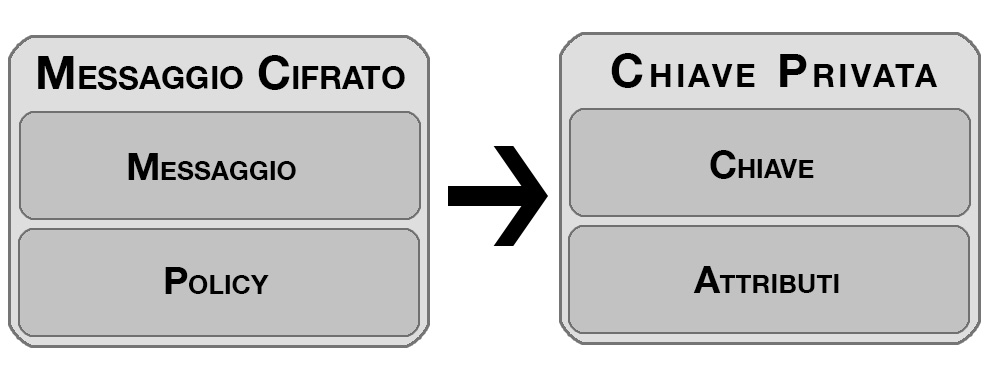
\includegraphics[keepaspectratio,width=\textwidth]{CT.jpg}\\
		{\small\scshape Chipertext Policy}
	\end{minipage}
	\hfill
	\begin{minipage}[c]{0.45\textwidth}
		\centering
		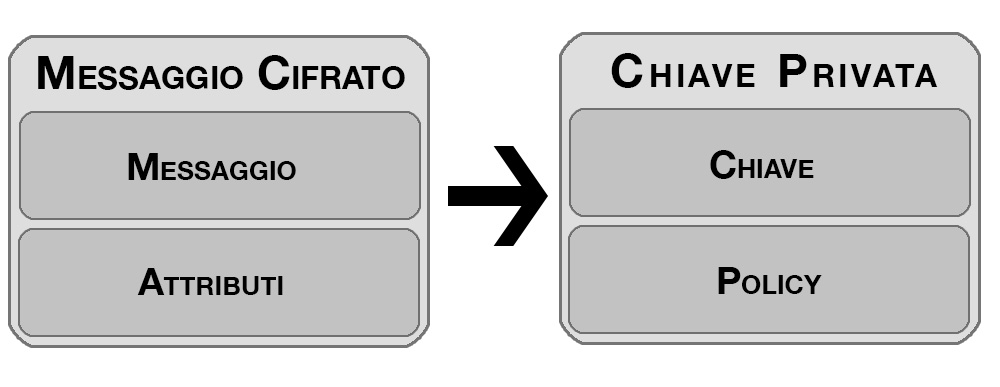
\includegraphics[keepaspectratio,width=\textwidth]{KP.jpg}\\
		{\small\scshape Key Policy}
	\end{minipage}
\vspace{0,8cm}
\end{minipage}

In entrambi i casi, possiamo caratterizzare\cite{maya3} queste famiglia in base ai gruppi su cui agisce la mappa bilineare :
\begin{itemize}
	\item $G_1 = G_2$ e di ordine $q$ primo
	\item $G_1 \neq G_2$ entrambi di ordine $q$ primo ed esiste un isomorfismo tra loro
	\item $G_1 \neq G_2$ entrambi di ordine $q$ primo e non esiste un isomorfismo tra loro
\end{itemize}	

Utilizzeremo il primo tipo dove $G_1 = G_2$ ed entrambi di ordine $q$ primo in uno schema \textbf{Key Policy ABE}

\newpage
\section{Struttura generale}

Consideriamo un insieme di parties $\{P_1, \cdots , P_n \}$ su cui costruiamo una gerarchia $\mathbb{A}$ che raccoglie le varie tipologie d'accesso che vogliamo garantire e verranno descritte come sottoinsiemi di parties.\\
In questo modo, un insieme $A$ è autorizzato dal sistema unicamente se è contenuto nella gerarchia $\mathbb{A}$.

Nel nostro caso, il ruolo dei parties viene preso dagli attributi.


\begin{defi}
Un \textbf{struttura d'accesso} è una collezione di sottoinsiemi non vuoti di parties $\mathbb{A} \subseteq 2^{\{ P_1,\cdots,P_n \}} \setminus \{ \emptyset \}$.\\
Gli insiemi di $\mathbb{A}$ sono detti \textbf{insiemi autorizzati} e gli insiemi non in $\mathbb{A}$ sono detti \textbf{insiemi non autorizzati}.
\end{defi}

\begin{defi}
Una collezione $\mathbb{A} \subseteq 2^{\{P_1,\cdots,P_n\}}$ è detta \textbf{monotona} se per ogni $B,C$ sottoinsiemi di $\{ P_1,\cdots,P_n \}$ con $B \subseteq C$ e $B \in \mathbb{A}$ allora $C \in \mathbb{A}$.
\end{defi}

Nella nostra trattazione useremo sempre strutture d'accesso monotone.\\[0.8cm]




La struttura di uno schema KP-ABE prevede 4 algoritmi:
\begin{description}
\item[Impostazione :] Algoritmo con in ingresso unicamente i parametri di sicurezza impliciti del sistema. Ritorna le chiavi publiche \pk e la chiave principale \mk.
\item[Criptare :] Algoritmo che riceve un messaggio $m$, un insieme di attributi $\gamma$ e i parametri pubblici \pk. Ritorna il messaggio criptato $E$.
\item[Generazione chiavi :] Algoritmo che partendo da una struttura d'accesso $\mathbb{A}$, la chiave principale \mk e le chiavi pubbliche , fornisce una chiave di decifrazione $D$.
\item[Decifrare :]L'algoritmo riceve in input il messaggio criptato $E$ che è stato criptato in un insieme d'attributi $\gamma$, la chiave di decifrazione $D$ per l'accesso alla struttura $\mathbb{A}$ e i parametri pubblici \pk.\\
Ritornerà il messaggio $M$ se $\gamma \in \mathbb{A}$
\end{description}

\vspace{0.8cm}

Per poter valutare la sicurezza del sistema, si definisce un modello \textbf{selective-set (game)} che procede in questo modo:
\begin{description}
\item[Inizializzazione :] L'avversario \evil{E} dichiara l'insieme degli attributi $\gamma$ su cui vuole esser sfidato.
\item[Impostazione :] Lo sfidato \evil{C} esegue il setup del sistema KP-ABE e fornisce ad \evil{E} i parametri pubblici all'avversario.
\item[Fase 1 :] \evil{E} ha il permesso di interrogare \evil{C} per tutte le chiavi private delle strutture $\mathbb{A}_j$ dove $\gamma$ non è un accesso autorizzato.
\item[Sfida :] L'avversario \evil{E} invia due messaggi di ugual lunghezza $M_0$ ed $M_1$.\\
\evil{C} lancia una moneta binaria $b$ e cripta il messaggio $M_b$ con $\gamma$. Il cifrato è mandato a \evil{E}.
\item[Fase 2 :] Come fase 1.
\item[Guess :] \evil{E} ritorna una risposta $b^\prime$ rispetto a $b$
\end{description}

Mediante questo gioco, il vantaggio dell'avversario \evil{A} è definito come \[\left\lvert \mathbb{P}(b = b^\prime) - \frac{1}{2}\right\rvert\]

\begin{defi}
Uno schema KP-ABE è \textbf{sicuro} in un modello di sicurezza selective-set se ogni avversario a tempo polinomiale ha al massimo un vantaggio trascurabile nel gioco selective-set.
\end{defi}

dove definiamo
\begin{defi}
Tratto da \cite[Def~1.2]{crittoalice}.\\
Un avversario \evil{A} è detto \textbf{avversario a tempo polinomiale} se usa nella sua logica un certo grado di randomicità (\evil{A} è quindi probabilistico) e se l'esecuzione di \evil{A} termina in un numero di passi $t$ polinomiale rispetto alla lunghezza dell'input. 
\end{defi}

\vspace{0.5cm}
Considerando la mappa bilineare non degenere $e:G_1 \times G_1 \rightarrow G_2$, il nostro obbiettivo è di dimostrare

\begin{assu}[Decisionale Bilineare Diffie - Hellman]
Siano $a,b,c,z \in \mathbb{Z}_p$ scelti casualmente e sia $g$ un generatore di $G_1$ ciclico dove $p$ è l'ordine di $G_1$\\
Nessun algoritmo $\mathcal{B}$ a tempo polinomiale probabilistico può distinguere tra le tuple
\[ (A = g^a , B = g^b , C = g^c , e(g,g)^{abc}) \qquad (A = g^a , B = g^b , C = g^c , e(g,g)^{z}) \]
con al più un vantaggio trascurabile.\\
Il vantaggio di $\mathcal{B}$ è
\[ \left\lvert \mathbb{P}\left( \mathcal{B}(A,B,C,e(g,g)^{abc}) = 0 \right) - \mathbb{P}\left( \mathcal{B}(A,B,C,e(g,g)^{z}) = 0 \right) \right\rvert \]
dove la probabilità è \emph{considerata} sulla scelta casuale di $a,b,c,z \in \mathbb{Z}_p$ e la scelta casuale di $\mathcal{B}$.
\end{assu}
\newpage
\subsection{Costruzione del sistema} 

% Le chiavi private sono identificate da una struttura d'accesso ad albero dove ogni nodo interno è una funzione di soglia e le foglie sono gli attributi. \\
Un utente potrà decifrare un messaggio cifrato con una data chiave privata unicamente se il messaggio soddisfa la policy d'accesso della chiave.\\[0.3cm]

\begin{defi}\-\\
Sia \evil{T} un \textbf{albero} rappresentante la nostra struttura d'accesso $\mathbb{A}$.\\[0.1cm]
Ogni non-foglia dell'albero rappresenta una funzione di soglia, descritta dai suoi figli e da un valore di soglia.\\
Se $\num_x$ è il numero di figli di un dato nodo $x$ e $k_x$ e il suo valore di soglia, allora $0 < k_x \leq \num_x$.\\
Quando $k_x = 1$, la funzione agisce come un OR mentre per $k_x = \num_x$ essa diventa una AND.\\
Ogni foglia è descritta dal suo attributo e una soglia di $k_x = 1$.\\[0.2cm]
Nel nostro albero ci è possibile definire un ordine rispetto ai figli di un nodo $x$ che li ordina da $1$ a $\num_x$. Questi indici sono univocamente assegnati ai nodi per ogni chiave d'accesso arbitraria.
\end{defi}
\vspace{0.3cm}

Per semplificare il lavoro con gli alberi, definiamo delle funzioni:
\begin{itemize}
\item $\parent(x)$ : ci ritorna il genitore del nodo $x$.
\item $\att(x)$ : se $x$ è una foglia, ci fornisce il suo attributo.
\item $\inde(x)$ : fornisce l'indice dell'ordine del nodo $x$ rispetto al genitore $\parent(x)$
\item $\mathcal{T}_x$ : è il sottoalbero di \evil{T} con radice $x$ 
\end{itemize}

\vspace{0.3cm}
A questo punto, creiamo un algoritmo che ci permetta di verificare se un dato insieme di attributi può accedere o meno nell'albero.
\vspace{0.5cm}

\textbf{ \large Soddisfare un albero d'accesso}\\[0.1cm]
Denotiamo con 
\begin{center}
$\mathcal{T}_x(\gamma) = 1$ se e solo se l'insieme d'attributi $\gamma$ soddisfa l'albero d'accesso $\mathcal{T}_x$
\end{center}
Calcoliamo $\mathcal{T}_x(\gamma)$ in questo modo:
\begin{description}
\item[$x$ è una foglia :] \[\mathcal{T}_x(\gamma) = 1 \Leftrightarrow att(x) \in \gamma\]
cioè è garantito l'accesso se gli attributi della foglia sono presenti in $\gamma$
\item[$x$ non è una foglia :] \[\mathcal{T}_x(\gamma) = 1  \Leftrightarrow \# \{x^\prime \text{ figli di } x \quad|\quad \mathcal{T}_{x^\prime}(\gamma) = 1  \} \geq k_x\]
cioè viene garantito l'accesso unicamente se il numero di figli che autorizzano $\gamma$ sono almeno in numero la soglia del nodo $x$ 
\end{description}

\vspace{0.8cm}

Ora prendiamo un $G_1$ gruppo bilineare di ordine $p$ e sia $g$ un generatore di $G_1$.\\
%Un parametro di sicurezza $k$ determinerà la grandezza dei gruppi.\\ % Non è utile nella tesi e può esser richiamato
\begin{defi}\label{pairinge}
$e : G_1 \times G_1 \rightarrow G_2$ mappa bilineare che soddisfa :
\begin{enumerate}
\item $e$ è bilineare rispetto al prodotto
\[ \forall_{u,v \in G_1}, a,b \in \mathbb{Z}_p : e(u^a,v^b) = e(u,v)^{ab} \]
\item $e$ è non degenere \[e(g,g) \neq 1\]
\item $e$ è velocemente computabile
\end{enumerate}
\end{defi}

\vspace{0.8cm}

\textbf{\Large Creazione sistema}

\begin{description}
\item[Impostazione :]Definiamo l'universo di attributi $\mathcal{U} = \{1,\cdots,n\}$. Ora, per ogni attributo $i \in \mathcal{U}$, scegliamo uniformemente a caso un elemento $t_i$ di $\mathbb{Z}_p$. Allo stesso modo prendiamo un $y$.\\
I parametri pubblici \pk pubblicabili sono
\[ T_1 = g^{t_1} , T_2 = g^{t_2} , \cdots , T_n = g^{t_n} , Y = e(g,g)^y \]\label{pubchiavi}
mentre la chiave principale \mk è
\[ t_1 , t_2 , \cdots , t_n , y \]
\vspace{0.1cm}
\item[Criptare :] Partendo da $(M , \gamma, \text{ \pk })$, cripto $M \in G_2$ sotto un insieme di attributi $\gamma$ scegliendo un $s$ casualmente in $\mathbb{Z}_p$ e pubblico il testo cifrato come
\[ E = (\gamma , E^\prime = MY^s , \{E_i = T_i^s \}_{i\in\gamma}) \]
\vspace{0.1cm}
\item[Generazione chiavi :] Partendo da $( \mathcal{T} , MK )$, l'algoritmo ci fornisce una chiave capace di decifrare il messaggio rispetto a $\gamma$ se e solo se $\mathcal{T}(\gamma) = 1$ cioè $\gamma$ è un insieme di attributi autorizzato.
\begin{enumerate}
\item Scelgo un polinomio $q_x$ per ogni nodo $x$, incluse le foglie, dell'albero \evil{T}.\\
I polinomi sono scelti dall'alto al basso, partendo quindi dalla radice.
\item Per ogni nodo $x$, sia $d_x$ il grado del polinomio $q_x$ tale che $d_x = k_x - 1$ con $k_x$ valore di soglia del nodo.
\item Per il nodo principale $r$, fissiamo $q_r(0) = y$ ed altri $d_r$ punti per completare la definizione del polinomio $q_r$.
\item Per gli altri nodi, fissiamo $q_x(0) = q_{\parent(x)}(\inde(x))$ e scegliamo altri $d_x$ altri punti per completare il polinomio.
\item Per ogni foglia $x$, ritorniamo all'utente la chiave di decriptazione
\[ D_x = g^{\frac{q_x(0)}{t_i}} \qquad \text{ dove } i \in \att(x) \]
\end{enumerate}
L'insieme di tutte le chiavi di sopra forma la chiave di decriptazione $D$
\vspace{0.1cm}
\item[Decifrare :] Partendo da $(E,D)$. Definiamo il nostro metodo di decifrazione mediante un algoritmo ricorsivo:\\
Sia $\decrypt( E , D , x )$ in un elemento di $G_2$ oppure non è permesso calcolarlo e lo indicheremo con $\perp$.\\
Sia $i = \att(x)$.
\begin{itemize}
\item Se $x$ è una foglia
\[ \decrypt(E,D,x) = \begin{cases}
\perp \qquad \text{ se } i \notin \gamma\\
e(D_x,E_i) = e(g^{\frac{q_x(0)}{t_i}},g^{s\cdot t_i}) = e(g,g)^{q_x(0) \cdot s}
\end{cases} \]
\item Se $x$ non è una foglia :\\
Per ogni nodo figlio $z$ di $x$, $F_z = \decrypt(E,D,z)$.\\
Considero i coefficienti di Lagrange :
\[ \Delta_{i,S}(x) = \prod_{j \in S , j \neq i} \frac{x-j}{i-j} \]

Sia $S_x$\label{insiemedecript} un insieme arbitrario di dimensione $k_x$ di figli $z$ tali che $F_z \neq \perp$.\\
Se non esiste alcun insieme di questo tipo, allora la funzione ritorna $\perp$. Altrimenti
\begin{align*}
F_x &= \prod_{z \in S_x} F_z^{\Delta_{i,S_x^\prime}(0)} \qquad \text{ dove }
\begin{matrix}
i = \inde(x)\\
S^\prime_x = \{ \inde(z) : z \in S_x \}
\end{matrix}\\
&= \prod_{z \in S_x} (e(g,g)^{s \cdot q_z(0)})^{\Delta_{i,S_x^\prime}(0)}\\
&= \prod_{z \in S_x} (e(g,g)^{s \cdot q_{\parent(z)}(\inde(z))})^{\Delta_{i,S_x^\prime}(0)} \qquad \text{(per costruzione)}\\
&= \prod_{z \in S_x} e(g,g)^{s \cdot q_x(i) \cdot \Delta_{i,S_x\prime}(0)}\\
&= e(g,g)^{s \cdot q_x(0)} 
\end{align*}
Dove l'ultimo passaggio è stato svolto per interpolazione polinomiale:\\
consideriamo il polinomio
\[ P(t) = \sum_{i \in S^\prime_x} q_x(i) \Delta_{i,S^\prime_x}(t)\]
Notiamo che la cardinalità dell'insieme $ S^\prime_x$ è maggiore rispetto al grado di $q_x(t)$.\\
La valutazione di $P(t)$ nei punti di $S^\prime_x$ ci fornisce 
\[P(j) = \sum_{i \in S^\prime_x} q_x(i) \Delta_{i,S^\prime_x}(j) = \sum_{i \in S^\prime_x} q_x(i) \delta_{i,j} = q_x(j)\]
cioé la valutazione di $P$ corrisponde con quella di $q_x$ in esattamente $\# S^\prime_x = \deg q_x + 1$ punti.\\
Per questo, i due polinomi coincidono ed abbiamo $P(0) = q_x(0)$.
% \href{http://math.stackexchange.com/questions/685472/find-n-degree-polynomial-from-n1-points}{(Spiegazione formale)}

\item Per decifrare usiamo $\decrypt (E,D,r)$ dove $r$ è la radice dell'albero
\end{itemize}
Quel che si nota è che se soddisfiamo l'albero, $\decrypt (E,D,r) = e(g,g)^{ys} = Y^s$ e poiché $E^\prime = MY^s$, l'algoritmo semplicemente divide per $Y^s$ che ottiene dal calcolo e recupera il messaggio $M$.
\end{description}



\newpage

\subsection{Assunzione Diffie - Hellman}

\begin{thm}
Se un avversario può rompere lo schema in un modello ABE Selective-Set, allora un simulatore può esser costruito per giocare al gioco Decisional Bilinear Diffie Hellman con un vantaggio non trascurabile.
\begin{proof}
Per dimostrare il teorema, supponiamo esista un avversario \evil{A} a tempo polinomiale che può rompere lo schema con un vantaggio $\epsilon$.\\
Costruiamo quindi un simulatore \evil{B} capace di giocare al gioco D-BDH con un vantaggio di $\epsilon / 2$ in questo modo :\\[0,5cm]

Facciamo scegliere allo sfidante i gruppi $G_1, G_2$ con una mappa $e$ efficente e un generatore $g$.\\
Successivamente il simulatore lancia una moneta $\mu$ di cui risultato non viene rivelato allo sfidante.\\
Se $ \mu = 0$ allora viene scelto $(A,B,C,Z) = (g^a,g^b,g^c,e(g,g)^{abc})$ altrimenti $(A,B,C,Z) = (g^a,g^b,g^c, e(g,g)^z)$ per dei valori $a,b,c,z$ casuali.\\
Assumiamo l'insieme degli attributi \evil{U} definito.

\begin{description}
\item[Inizializzazione :] Il simulatore \evil{B} esegue \evil{A}. \evil{A} decide l'insieme degli attributi $\gamma$ su cui vuol esser sfidato.
\item[Setup :] Il simulatore \evil{B} fissa il parametro $Y= e(A,B) = e(g,g)^{ab}$.\\
Per ogni $i \in \mathcal{U}$, viene fissato $T_i$ come :
\begin{enumerate}
\item Se $i \in \gamma$ allora si sceglie casualmente $r_i \in \mathbb{Z}_p$ e fissiamo $T_i = g^{r_i}$
\item Altrimenti scegliamo casualmente $\beta_i$ e fissiamo $T_i = g^{\beta_i b} = B^{\beta_i}$
\end{enumerate}
Successivamente \evil{A} ritorna i parametri pubblici a \evil{B}
\item[Fase 1 :] \evil{A} esegue richieste di chiavi corrispondenti ad ogni albero d'accesso \evil{T} tale che $\gamma$ non soddisfa \evil{T}.\\
Supponiamo che \evil{A} faccia una richiesta per un albero \evil{T} dove $\mathcal{T}(\gamma) = 0$.\\
Per generare la chiave, \evil{B} deve assegnare un polinomio $Q_x$ di grado $d_x$ per ogni nodo $x$ di \evil{T}.\\
Definiamo quindi due casistiche :
\begin{itemize}
\item $\polysat (\mathcal{T}_x , \gamma, \lambda_x )$ : questa procedura viene eseguita se $\mathcal{T}_x(\gamma) = 1$ cioè viene soddisfatto l'albero. $\lambda_x$ è un valore in $\mathbb{Z}_p$.\\
Per prima cosa fissiamo un polinomio $q_x$ di grado $d_x$ per il nodo radice $x$ tale che $q_x(0) = \lambda_x$ e setta in maniera casuale gli altri valori per completare $q_x$.\\
Successivamente, per ogni figlio $x^\prime$ di $x$, viene richiamata la procedura $\polysat(\mathcal{T}_{x^\prime}, \gamma, q_x(\inde(x^\prime))$ così da ottenere $q_{x^\prime} (0) = q_x (\inde(x^\prime))$.
\item $\polyunsat(\mathcal{T}_x, \gamma , g^{\lambda_x})$ : questa procedura viene eseguita se $\mathcal{T}_x (\gamma) = 0$ cioé quando non viene soddisfatto l'albero. $g^{\lambda_x} \in \mathbb{G}_1$.\\
Viene fissato un polinomio $q_x$ di grado $d_x$ per il nodo $x$ tale che $q_x(0) = \lambda_x$. Siccome $\mathcal{T}_x(\gamma) = 0$, non più di $d_x$ figli soddisfano l'albero.\\
Sia quindi $h_x \leq d_x$ il numero di figli che soddisfano l'albero in $x$ e per questi viene scelto a caso un $\lambda_{x^\prime} \in \mathbb{Z}_p$ e fissiamo $q_{x^\prime}(0) = \lambda_{x^\prime}$. Successivamente vengono fissati casualmente i restanti $d_x - h_x$ punti di $q_x$ per completare il polinomio.\\
L'algoritmo procede nella definizione dei polinomi per ogni nodo figlio $x^\prime$ di $x$ come
\begin{itemize}
\item $\polysat(\mathcal{T}_{x^\prime} , \gamma , q_x(\inde(x^\prime)))$ se $x^\prime$ è un nodo soddisfacente $\gamma$.\\
Da osservare che in questo caso siamo a conoscenza di $q_x(\inde(x^\prime))$.
\item $\polyunsat(\mathcal{T}_{x^\prime} , \gamma , g^{q_x(\inde(x^\prime))})$ se $x^\prime$ non è un nodo soddisfacente $\gamma$.\\
Da osservare che in questo caso siamo a conoscenza unicamente di $g^{q_x(\inde(x^\prime))}$ per interpolazione a partire da $g^{q_x(0)}$.
\end{itemize}
Osserviamo che anche in questo caso $q_{x^\prime}(0) = q_x(\inde (x^\prime))$ per ogni nodo figlio $x^\prime$ di $x$.
\end{itemize}
Per fornire gli accessi alla struttura \evil{T}, il simulatore esegue $\polyunsat(\mathcal{T},\gamma,A)$ per definire un polinomio $q_x$ per ogni nodo $x$ di \evil{T}.\\
Per ogni foglia $x$ di \evil{T} conosciamo $q_x$ completamente se $x$ soddisfa $\gamma$, altrimenti conosciamo unicamente $g^{q_x(0)}$.\\
Inoltre $q_r(0) = a$.\\
Il simulatore ora definisce $Q_x(\cdot) = b q_x( \cdot)$ per ogni nodo $x \in \mathcal{T}$.\\
Osserviamo che così otteniamo $y = Q_r(0) = ab$. La chiave corrispondente per ogni foglia è data utilizzando il suo polinomio come segue. Sia $i = \att(x)$.
\[ D_x = \begin{cases}
g^{\frac{Q_x(0)}{t_i}} = g^{\frac{b q_x(0)}{r_i}} = B^{\frac{q_x(0)}{r_i}}  \qquad \text{ se } i \in \gamma\\
g^{\frac{Q_x(0)}{t_i}} = g^{\frac{b q_x(0)}{b \beta_i}} = g^{\frac{q_x(0)}{\beta_i}} \qquad \text{ altrimenti}
\end{cases} \]
In questo modo il simulatore \evil{B} riesce a costruire le chiavi private per gli accessi alla struttura \evil{T}.
\item[Sfida :] L'avversario \evil{A} invia due messaggi $m_0$ e $m_1$ al simulatore \evil{B}.\\
\evil{B} lancia una moneta binaria equiprobabile $\nu$ e ritorna il cifrato di $m_\nu$ come
\[ E = (\gamma , E^\prime = m_\nu Z , \{ E_i = C^{r_i} \}_{i \in \gamma} ) \]
Se $\mu = 0$ allora $Z = e(g,g)^{abc}$.\\
Da questo abbiamo che $s = c$ cioé $Y^s = (e(g,g)^{ab})^c = e(g,g)^{abc}$ e $E_i = (g^{r_i})^c = C^{r_i}$. Otteniamo quindi una valida cifratura del messaggio $m_\nu$.\\
Se $\mu = 1$ allora $E^\prime = m_\nu e(g,g)^z$ è un elemento casuale di $\mathbb{G}_2$ e non è così possibile avere informazioni su $m_\nu$ data l'arbitrarietà di $z$.
\item[Fase 2 :] Viene ripetuto quel che è stato fatto nella Fase 1.
\item[Guess :] \evil{A} manda un ipotesi $\nu^\prime$ di $\nu$. Se $\nu^\prime = \nu$ allora \evil{B} ritornerà $\mu^\prime = 0$ per indicare che è stata data una BDH-tupla valida, $\mu^\prime = 1$ se la tupla è casuale.
\end{description}

Come si può vedere, la costruzione del simulatore è uguale a quella dello schema originale.\\[0.5cm]

Calcoliamo ora il vantaggio dello sfidante nel selective-set game che risulta essere
\[\mathbb{P}[ \mu = \mu^\prime] - \frac{1}{2} \]
Nel caso $\mu = 1$, l'avversario non riceve informazioni su $\nu$.
Quindi abbiamo che $\mathbb{P}[\nu \neq \nu^\prime | \mu = 1] = \frac{1}{2}$.
Siccome \evil{A} cerca di indovinare $\mu^\prime = 1$ quando $\nu^\prime \neq \nu$, abbiamo che $\mathbb{P}[\mu = \mu^\prime| \mu = 1] = \frac{1}{2}$\\[0.2cm]
Se $\mu = 0$, \evil{A} vede il cifrato di $m_\nu$. Il vantaggio è $\epsilon$ dà ipotesi.\\
Quindi $\mathbb{P}[\nu \neq \nu^\prime | \mu = 0] = \frac{1}{2} + \epsilon$.\\
Siccome viene ipotizzato $ \mu = \mu^\prime$ quando $\nu \neq \nu^\prime$, abbiamo $\mathbb{P}[\mu = \mu^\prime | \mu = 0] = \frac{1}{2} + \epsilon$.\\[0.2cm]
A questo punto, il vantaggio complessivo di un simulatore che gioca al DBDH è 
\[ \frac{1}{2} \mathbb{P}[\mu = \mu^\prime | \mu = 1] + \frac{1}{2}\mathbb{P}[\mu = \mu^\prime | \mu = 0] - \frac{1}{2}  = \frac{1}{2}\left( \frac{1}{2} + \epsilon \right) + \frac{1}{2}\frac{1}{2} - \frac{1}{2} = \frac{1}{2} \epsilon\]
\end{proof}
\end{thm}





\chapter{Esempio Concreto}

Vogliamo costruire uno schema KP-ABE.\\
Suddivideremo la costruzione nei vari passaggi più delicati per analizzarli in maniera più precisa.

\section{Scelta della mappa bilineare}

\begin{itemize}
	\item Si può parlare del pairing di Weil e Tate anche se sforano entrambi sulle curve elittiche per costruire il pairing
	\item Costruzione base partendo da $C_p \times C_p \rightarrow C_p$ che manda $e(g,g) = g$ dove $g$ è un generatore
\end{itemize}

\section{Costruzione dell'albero d'accesso}

\begin{itemize}
	\item Mostrare l'albero che utiliziamo per il nostro esempio e la struttura d'accesso
	\item Valutare se è un punto così delicato
\end{itemize}

\section{Generazione e distribuzione delle chiavi}

\begin{itemize}
	\item La ``Impostazione , Criptare , Generazione Chiavi'' dello schema
	\item Generazione polinomi dell'albero 
\end{itemize}

\section{Visione d'insieme}

Grafo d'utilizzo e spostamento delle chiavi/messaggi (può esser interessante?)

\chapter{Conclusioni}
\section{Sicurezza}
\textbf{Qualità sicurezza a discapito della difficoltà computazionale. Un possibile commento sulla possibile resa in opera del sistema.}
\section{Breaking the code}
\textbf{Accenni su un possibile modo per decifrare la struttura (necessità di utilizzo di un metodo di DiscreteLogarithm sui gruppi).}
\section{Problemi aperti}
\textbf{Sono presenti nel paper dei problemi aperti. Alcuni sono relativi ad altri paper della stessa famiglia di metodi ABE. Devo ancora valutare se si riescono a inserire senza inserire nuovi concetti rispetto a quelli che tratto.}




\bibliographystyle{plainnat}
\bibliography{biblio}


\end{document}